\chapter{Data Fusion Algorithm}
\label{ch:method}

這個是插入圖片的範例, 圖片都放在img資料夾裡面. 檔案格式有支援: JPG, PNG, PDF, EPS. 就使用自己習慣的繪圖工具, 比較常見的應該就是power point!? power point可以把繪圖區另存成JPG, PNG, 還有SVG (新版才有, 我用的office 2016沒有這選項 QQ). SVG可以再轉成PDF, 這樣圖片縮放還是會很清楚, 可以把範例的兩張圖片都放大來看, 應該可以看出差別. 我個人都是用visio來畫圖, 可是都找不到替代工具, 如果有好用的繪圖工具麻煩分享交流一下 QQ 也看過蠻多人用draw.io, 只是這個用起來不太順手. orz
圖片出現的位置是由latex去決定, 有時候會出現在奇怪的地方, 這時候只能多爬文、嘗試各種參數, 或者把整段圖片code放在前面試試看.

overleaf上有插入圖片的介紹: https://www.overleaf.com/learn/latex/Inserting\_Images


    \begin{figure}
      \centering
      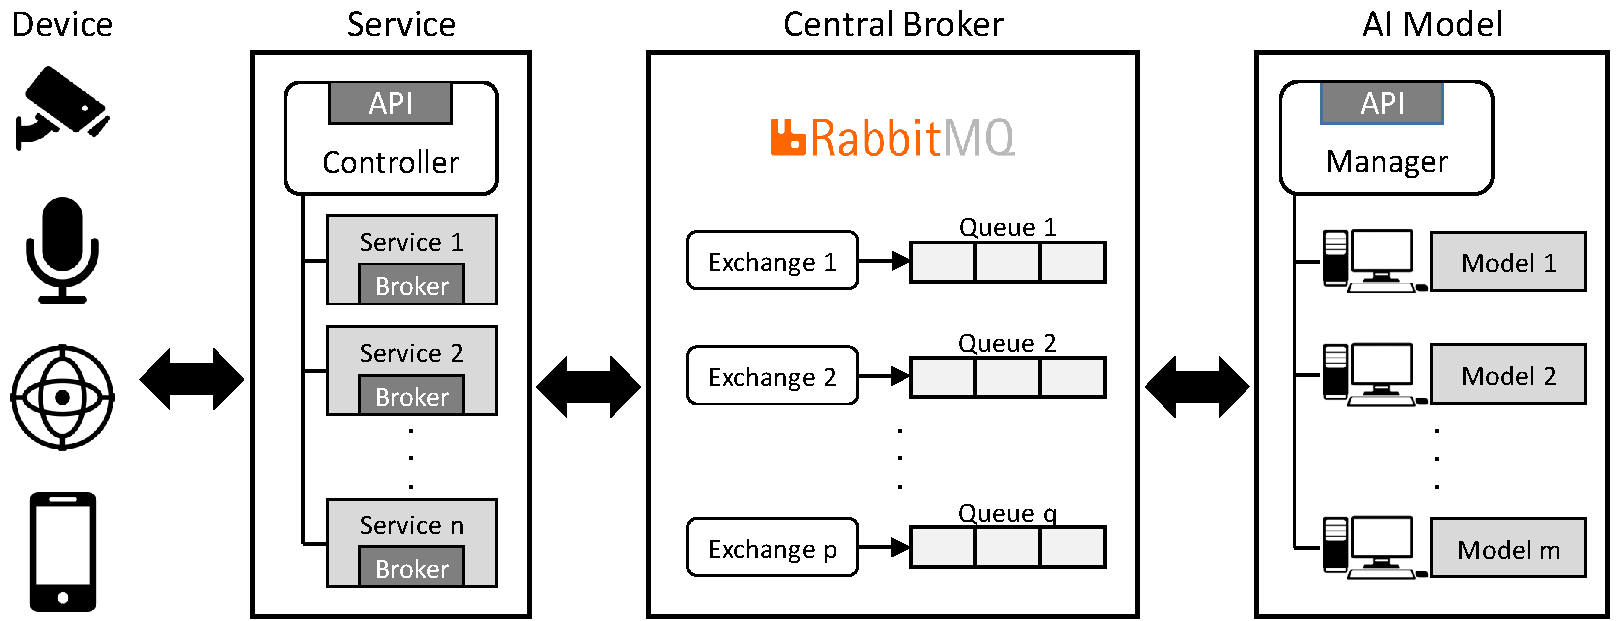
\includegraphics[width=1\columnwidth]{img/1.system_architecture.pdf}
      \caption{PDF圖檔範例.} 
      \vspace{-0.4cm}
      \label{fig:system_architecture}
    \end{figure}

\begin{figure}[htb]
	\centering
	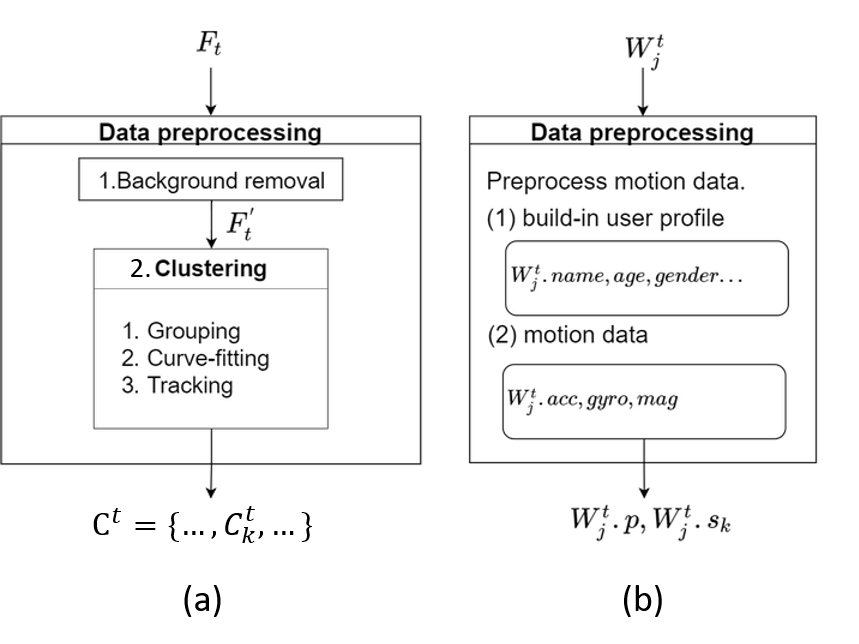
\includegraphics[width=0.6\textwidth]{img/data_preprocessing.png}
	\caption{PNG example.}
	\label{fig:model}
\end{figure}

\section{Data Preprocessing}
\label{sec:SMA}
An example for section. Fig~\ref{fig:system_architecture} is PDF. Fig~\ref{fig:model} is PNG.


\subsection{2D LiDAR Data}
An example for subsection. 寫中文就是 圖~\ref{fig:system_architecture} 跟圖~\ref{fig:model}.
